\documentclass[a4paper]{proc}

\usepackage{biblatex}
\usepackage{graphicx}

\addbibresource{references.bib}

\renewcommand*{\bibfont}{\raggedright}

\begin{document}

  \title{GDP Individual Report}
  \author{James Robinson\\\texttt{jr4e09@soton.ac.uk}}
  \maketitle

  \begin{abstract}
  \end{abstract}

  % Hypothesis: it's difficult for small companies to get into IaaS because of the associated costs, but building PaaS services on top of existing IaaS ones is feasible with little initial investment.

  % About 500 words per section

  \section{The importance of the idea}

  % What is cloud computing and why is it important?
  % What is the distinction between public, private and hybrid clouds, and which are we talking about here?
  % What are IaaS and PaaS and why are they useful?

  \begin{figure}
    \centering
    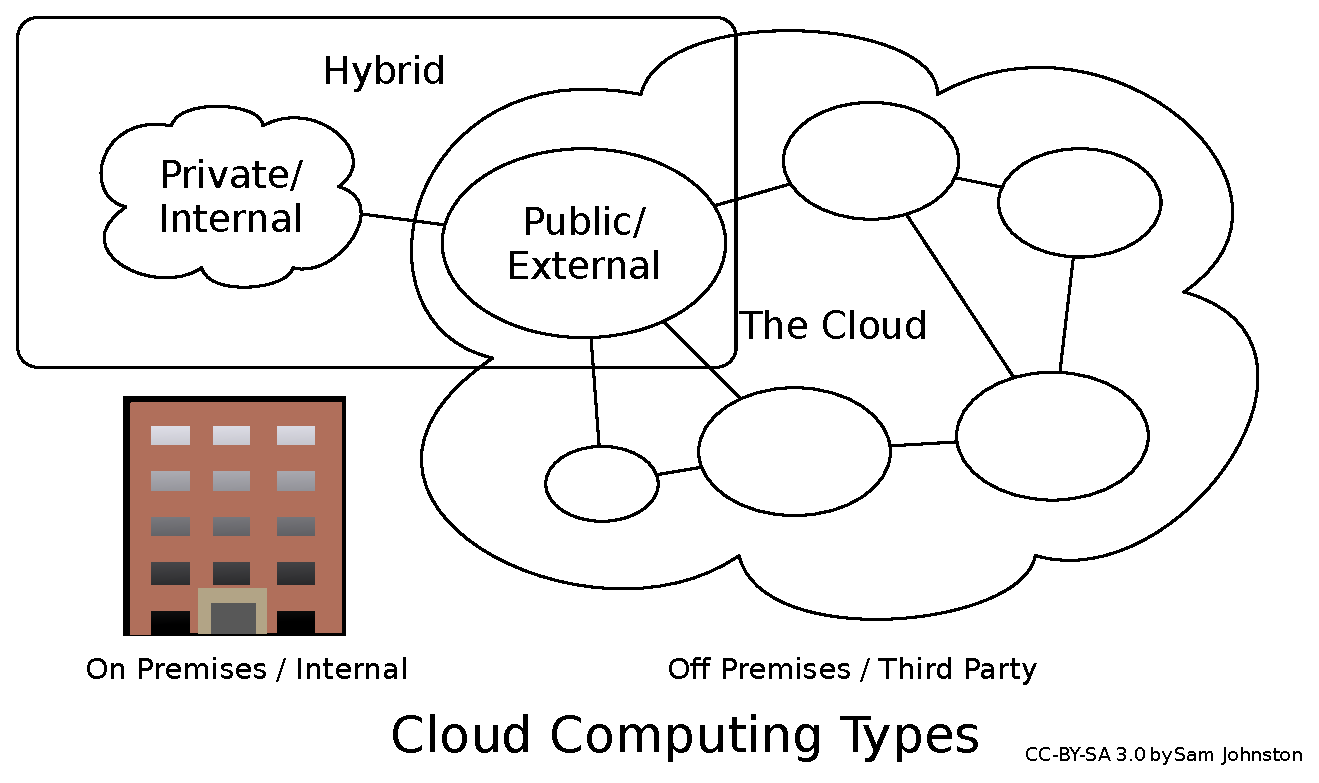
\includegraphics[width=\columnwidth]{figures/Cloud_computing_types.eps}
    \caption{Diagram showing three main types of cloud computing (public/external, hybrid, private/internal) \cite{Joton2009}}
    \label{fig:cloud_computing_types}
  \end{figure}

  The most fundamental type of cloud computing service is known as \emph{Infrastructure as a Service}, or IaaS. IaaS providers offer servers (either physical or virtual) on an on-demand basis, usually charging a fixed price per unit of time the server is used. IaaS providers frequently complement these servers with additional services such as block storage (e.g. virtual disks), object storage (e.g. key-value stores), load balancing, or additional IP addresses, again charging a fixed sum per unit of time the additional services are used. IaaS services are extremely valuable because they abstract away the physical infrastructure (servers, switches, routers, etc.), allow servers to be dynamically provisioned and de-provisioned to meet demand in real-time, and replace the large initial investment for the purchase of physical hardware with smaller incremental payments based on usage.

  A higher-level cloud computing model is known as \emph{Platform as a Service}, or PaaS. PaaS providers offer complete platforms for the deployment of applications, and automatically manage the provisioning of the underlying infrastructure on behalf of the application. This complete platform typically consists of an operating system, a runtime environment for one or more programming languages, a database server, one or more web servers and a load balancer. PaaS services are extremely valuable because they allow application developers to deploy their application without having to worry about provisioning and maintaining the underlying infrastructure or the software used to host the application.

  % Identify a technology market sector and identify the key players that operate in it.
  %    Market sector: public cloud computing service providers (not software, not private cloud)
  % Identify at least 2 competing products or services and discuss their target customer’s requirements and how these products/services address these needs.
  % You should argue your own opinion as to whether they are successful.
  % It can be useful to research competitors who have failed in the market to provide evidence

  % IaaS: VMs, servers, storage, load balancing, etc. providers
  % PaaS: runtime, database, web server, etc. providers

  % IaaS only: VMWare vCloud Air
  % IaaS and PaaS providers: Amazon Web Services, Microsoft Azure, HP Helion
  % PaaS only: Heroku, Red Hat OpenShift, Google App Engine, Engine Yard, IBM Bluemix

  \section{The importance of the market}

  % Using your original examples (and/or others) explain how market and distribution are important.
  % For example, how big is the market, what strategies are used to access the market
  %   (low price/high volume, free download/in-app purchase, monopolisation, or a platform for 3rd party competition)

  \section{Protection}

  % Explain why barriers to entry to a market are important, what these barriers can look like eg patents and how companies can protect their ideas and markets.
  % Again you can use your original example companies, or you can introduce new examples.

  % Barrier for entry for IaaS providers is upfront costs: you need to buy and manage a large number of physical servers. Amazon pretty much have the monopoly
  % Barrier for entry for PaaS providers is lesser since you can simply rent virtual servers. Because of the lower barrier for entry there are far more companies competing in this sector.
  % Some PaaS providers chose to only provide a specific ecosystem for example .NET, but that reduces the size of your target market

  \section{Finance}

  % Describe how technology companies can be financed and what sort of idea requires what sort of finance.
  % Give examples to support your hypotheses. (Examples might include bank loans, venture capital, crowdfunding, payment in advance from a customer)

  % Amazon
  %   Already invested in server infrastructure for their own service, and already had enormous amounts of capital
  % Microsoft
  % Engine Yard
  %   In January 2008, Engine Yard received an investment of $3.5 million from Benchmark Capital. Some industry commentators interpreted this as an investment in Ruby on Rails.
  %     http://www.techcrunch.com/2008/01/11/benchmark-bets-on-ruby-on-rails-with-35-million-investment-in-engine-yard/
  %   In July 2008, Engine Yard secured an additional $15 million from a combination of Benchmark Capital, New Enterprise Associates, and Amazon.
  %     http://ostatic.com/blog/engine-yard-secures-15-million-in-funding
  %  In October 2009, Engine Yard received an additional $19 million in funding from a combination of Benchmark Capital, New Enterprise Associates, Amazon, Bay Partners, Presidio Ventures and DAG Ventures, for a total of $37.5 million in funding.
  %  In November 2012, Oracle Corporation announced that it made a strategic minority investment in Engine Yard. Financial details of the investment were not disclosed. Engine Yard continues to operate as an independent company.
  % Heroku
  %   Heroku was acquired by Salesforce.com in 2010.
  %     http://news.heroku.com/news_releases/salesforcecom-signs-definitive-agreement-to-acquire-heroku

  \section{Survival}

  % What strategies can technology companies use to ensure their survival?
  % Look for examples where companies haven’t survived and maybe should have.
  % Likewise look for examples of companies who are implementing survival strategies

  \section{Other issues}

  % Look at other ideas that can affect market performance or opportunities eg legislation, key staff/knowledge, standards

  \section{Conclusion}

  \printbibliography

\end{document}
